\documentclass[letterpaper, twoside, 12pt,memoire]{thETS}
\usepackage{amsmath}
\usepackage{amsfonts}
\usepackage{amssymb}
\usepackage[utf8]{inputenc}
\usepackage{graphicx}
\usepackage{color}
\usepackage[T1]{fontenc}
\usepackage{subfigure}
\usepackage{setspace}
\usepackage{todonotes}
\usepackage{varwidth}
\usepackage{float}
\usepackage[section]{placeins}
\usepackage[round]{natbibETS}
\usepackage[mathcal]{euscript}
\usepackage{enumerate}

\hyphenpenalty=5000
\tolerance=1000

\newcommand{\fig}[1]{figure~\ref{#1}}
\newcommand{\bul}{$\quad\bullet$~~}
\newcommand{\ang}[1]{(\textit{#1})}
\newcommand{\sect}[1]{section~\ref{#1}}

\newcommand{\LT}[1]{%
	{
	\todo[inline,color={red!33!green!33!blue!33}]{%
	\textbf{[LT]:}~#1}
	}}
	
\newcommand{\SC}[1]{%
	{
	\todo[inline,color={red!100!green!33!}]{%
	\textbf{[SC]:}~#1}
	}}
%DIF PREAMBLE EXTENSION ADDED BY LATEXDIFF
%DIF UNDERLINE PREAMBLE %DIF PREAMBLE
\RequirePackage[normalem]{ulem} %DIF PREAMBLE
\RequirePackage{color}\definecolor{RED}{rgb}{1,0,0}\definecolor{BLUE}{rgb}{0,0,1} %DIF PREAMBLE
\providecommand{\DIFadd}[1]{{\protect\color{blue}\uwave{#1}}} %DIF PREAMBLE
\providecommand{\DIFdel}[1]{{\protect\color{red}\sout{#1}}}                      %DIF PREAMBLE
%DIF SAFE PREAMBLE %DIF PREAMBLE
\providecommand{\DIFaddbegin}{} %DIF PREAMBLE
\providecommand{\DIFaddend}{} %DIF PREAMBLE
\providecommand{\DIFdelbegin}{} %DIF PREAMBLE
\providecommand{\DIFdelend}{} %DIF PREAMBLE
%DIF FLOATSAFE PREAMBLE %DIF PREAMBLE
\providecommand{\DIFaddFL}[1]{\DIFadd{#1}} %DIF PREAMBLE
\providecommand{\DIFdelFL}[1]{\DIFdel{#1}} %DIF PREAMBLE
\providecommand{\DIFaddbeginFL}{} %DIF PREAMBLE
\providecommand{\DIFaddendFL}{} %DIF PREAMBLE
\providecommand{\DIFdelbeginFL}{} %DIF PREAMBLE
\providecommand{\DIFdelendFL}{} %DIF PREAMBLE
%DIF END PREAMBLE EXTENSION ADDED BY LATEXDIFF

\begin{document}

\DIFdelbegin %DIFDELCMD < \begin{chapter}{L'état de l'art de la détection de la détérioration visuelle
%DIFDELCMD < dans le domaine des pixels}
%DIFDELCMD < %%%
\DIFdelend \DIFaddbegin \begin{chapter}{Revue de la littérature}
\DIFaddend Dans ce chapitre, nous faisons état de la littérature sur les approches de
détection de la détérioration visuelle. Il ne s’agit pas ici d’une simple
énumération, mais bien, d’une suite logique d’ouvrages permettant de comprendre,
l’introduction et l’évolution de plusieurs concepts fondamentaux, sur lesquels
reposent notre contribution.

La détection de la détérioration visuelle \DIFdelbegin \DIFdel{sert à identifier la dégradation
visuelle engendrée suite au décodage }\DIFdelend \DIFaddbegin \DIFadd{est possible uniquement si le contenu
}\DIFaddend de paquets corrompus \DIFdelbegin \DIFdel{. Pour décoder ces
paquets}\DIFdelend \DIFaddbegin \DIFadd{peut être décodé. Pour ce faire}\DIFaddend , le décodeur du canal de
transmissions doit interagir avec le décodeur vidéo (source)\DIFdelbegin \DIFdel{, afin d'identifier et de rendre disponible les paquets corrompus}\DIFdelend . Ce type
d'interaction porte le nom de \textit{Joint Source Channel Decoding}. Notre
prologue, \sect{sect-prologue}, expose les origines du \textit{Joint Source
Channel Decoding}. La \sect{sect-SourceChannel} offre un compte rendu des
notions du \textit{Joint Source Channel Decoding} qui s'appliquent
spécifiquement au transport de séquences vidéo. Les améliorations apportées à
une de ces notions, l'analyse syntaxique, sont présentées à la
\sect{sect-SyntaxeAnalysis}. Finalement, à la \sect{sect-Combined}, les
approches combinant l'analyse syntaxique à la détection de la détérioration
visuelle dans le domaine des pixels sont décrites.


\begin{section}{Prologue}
\label{sect-prologue}
Dans son ouvrage \textit{A Mathematical Theory of Communication},
\citet{Shannon1948} explique sous l'allégorie ingénieuse du télégraphe, la
notion même du \textit{Joint Source Channel Decoding}. L'usage d'un langage
redondant, tel l'anglais, comme encodage pour le télégraphe a l'avantage d'être
résistant aux erreurs du canal de transmissions. Le contexte du message permet
la reconstruction des mots, même si plusieurs lettres de ceux-ci sont bruitées
\citep[p.~24]{Shannon1948}.

En \citeyear{Modestino1979}, \citeauthor{Modestino1979} sont les premières personnes à
proposer d'utiliser le \textit{Joint Source Channel Decoding} pour améliorer le
transport d'images numériques. Déjà à cette époque, \citeauthor{Modestino1979}
déplorent le gaspillage de bande passante introduit par les stratégies de
résilience aux erreurs. Un gaspillage qui, 30 ans plus tard, est toujours
présent sur les réseaux sans fil \citep[p.1]{Duhamel2010}.

\begin{figure}
\fbox{\DIFdelbeginFL \DIFdelFL{
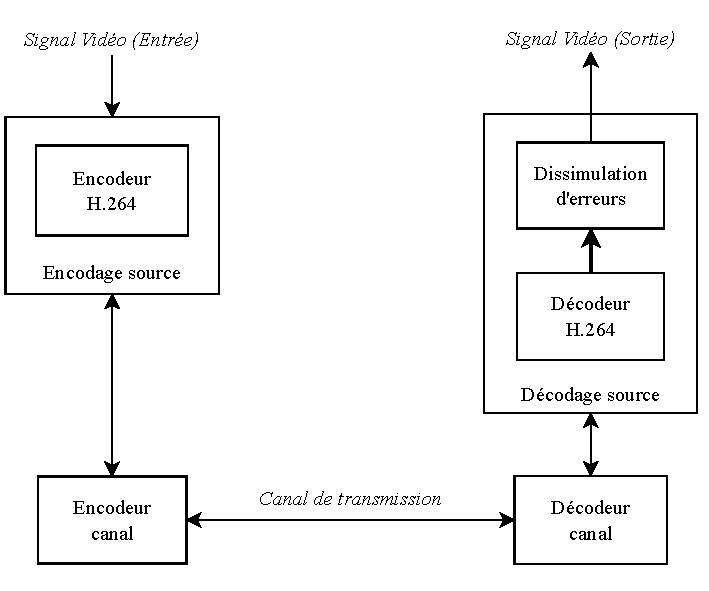
\includegraphics{images/VideoCommunication.pdf}
}\DIFdelendFL \DIFaddbeginFL \DIFaddFL{
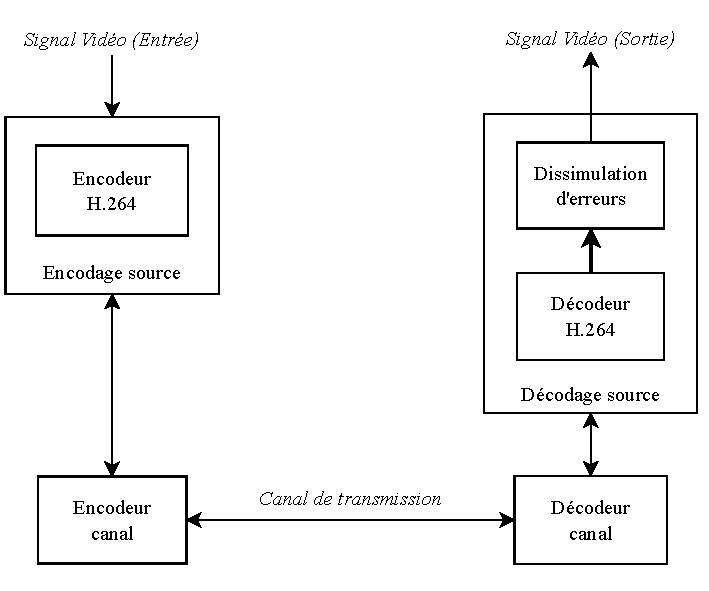
\includegraphics[width=0.65\linewidth]{images/VideoCommunication.pdf}
}\DIFaddendFL }
\caption{Diagramme à blocs des composantes liées au transport de séquences
vidéo.\\Adaptée de \citet[p.~976]{Wang1998}}
\label{fig-VideoCommunication}
\end{figure}

\DIFdelbegin \DIFdel{Avant de poursuivre, commençons par décrire les composantes liées au
\textit{Joint Source Channel Decoding}. La }%DIFDELCMD < \fig{fig-VideoCommunication} %%%
\DIFdel{résume
les étapes et interactions du \textit{Joint Source Channel Decoding}. Tout
d'abord, l'encodeur H.264 retire la redondance d'un signal vidéo. Par la suite,
l'encodeur du canal va empaqueter le contenu et insérer les mécanismes de
résilience à l'erreur nécessaires selon le canal de transmission. Notons l'ajout
de donnée redondante comme un des mécanismes de résilience à l'erreur. Dès la
réception de paquets chez le destinataire, le décodeur du canal dépaquette
ceux-ci et valide que leur contenu soit intact. À l'aide des données
dépaquetées, le décodeur H.264 reconstruit le signal vidéo. Cependant, si des
données sont manquantes, le décodeur H.264 fait appel à un algorithme de dissimulation d'erreurs pour permettre d'estimer les données manquantes.
}\DIFdelend \end{section}

\begin{section}{Établir le lien entre le décodeur vidéo et celui du canal de
transmission}
\label{sect-SourceChannel}
Les techniques de résilience aux erreurs sur des réseaux non fiables ont suscité
beaucoup d'intérêt dans les années 80 et 90. En \citeyear{Wang1998}, dans leur
revue sur les techniques de contrôle et de dissimulation d'erreurs lors du
transport de séquences vidéo \citep{Wang1998}, \citeauthor{Wang1998}
récapitulent, entre autres, l'état de l'art, de l'époque, des stratégies de
résilience aux erreurs. \citeauthor{Wang1998} présentent une multitude
d'approches. Parmi celles-ci, ils identifient un type d'approches qu'ils
qualifient d'approches de dissimulation par post-traitement effectué par le
décodeur \citep[Chap. 5]{Wang1998}. Ce type résume, de façon exacte, les
approches que nous présentons dans cet ouvrage. Leurs composantes sont
illustrées à la \fig{fig-VideoCommunication}. Parmi les approches de
dissimulation présentées en \citeyear{Wang1998}, on remarque:
\textit{Motion-Compensated Temporal Prediction}~\citep{Ghanbari1993},
\textit{Maximally Smooth Recovery}~\citep{Wang1993}, \textit{Projection onto
Convex Sets (POCS)}~\citep{Sun1995}, \textit{Spatial- and Frequency-Domain,
Interpolation}~\citep{Hemami1995} et \citep{Sun1992}.

Toutes ces approches de post-traitement, effectuées par le décodeur, présentées
par \citet{Wang1998}, supposent que les blocs endommagés sont connus.
Pratiquement, cette identification est accomplie en ignorant les paquets
corrompus, ce qui force le décodeur à dissimuler tous les blocs que contiennent
ces derniers même si un seul bloc est endommagé. Pour reprendre l'exemple du télégraphe, ceci revient à rejeter
l'ensemble des mots d'une phrase qui possède une lettre en erreur. Cela complique
grandement la compréhension du message. Ce nivellement par le bas, quoique plus
simple, est un exemple du gaspillage identifié par \citeauthor{Modestino1979},
où le décodeur de la source ne communique pas avec le décodeur du canal de
transport.

Le \textit{Joint Source Channel Decoding} \citep{Duhamel2010} cherche, à l'aide
de la logique de la source, à identifier précisément, où se trouve l'erreur dans
un ensemble de bits corrompus. Par exemple, pour l'encodage MPEG-4 Visual,
\citeauthor{Talluri1998} propose des règles permettant de vérifier la validité
de: la portée des vecteurs de mouvement, des codes entropiques décodés, la
portée des valeurs de coefficient DCT et du nombre de coefficients DCT afin
qu'il ne dépasse pas le nombre permis par la norme \citep{Talluri1998}. Une fois
l'erreur identifiée, il existe deux types de solutions possibles: la reconstruction et la dissimulation.

D'une part, la reconstruction vise à retrouver les valeurs originales des bits
corrompues à l'aide de modèles mathématiques complexes, comme présentée par
\citet{Duhamel2010}.

D'autre part, la dissimulation tente de décoder les paquets corrompus, et par la
suite, identifier et dissimuler la détérioration visuelle engendrée par cette
opération. L'article de \citeauthor{Ye2003}, parue en mai \citeyear{Ye2003},
présente un algorithme destiné au décodage d'images JPEG corrompues. Ce dernier
est capable d'identifier et classifier des blocs erronés, selon leurs
caractéristiques dans le domaine des pixels \citep{Ye2003}.

\citeauthor{Ye2003} définissent quatre mesures permettant d'identifier les blocs
erronés. La première est la validité de la valeur assignée à un pixel. Il s'agit
ici de déterminer si un pixel est dans un intervalle de données plausibles. Par
exemple~: pour les valeurs d'un pixel non signées de niveaux de gris assignées
sur huit bits, les valeurs possibles sont de 0 à 255. La deuxième mesure est
l'hétérogénéité des bordures de blocs horizontales mesurée à l'aide d'un filtre
Sobel. La troisième est l'hétérogénéité des bordures de blocs verticales, encore
une fois mesurée à l'aide d'un filtre Sobel. Dans d'autres oeuvres,
l'hétérogénéité en bordure de blocs est aussi connue sous le nom d'effet de
bloc. Le filtre Sobel est défini par les opérateurs suivants (horizontal et vertical respectivement)\DIFaddbegin \DIFadd{~}\DIFaddend :
\begin{equation}
S_h =
\begin{bmatrix}
-1 & 0 & 1\\
-2 & 0 & 2\\
-1 & 0 & 1\\
\end{bmatrix}, \quad
S_v =
\begin{bmatrix}
1 & 2 & 1\\
0 & 0 & 0\\
-1 & -2 & -1\\
\end{bmatrix}.
\end{equation}
La dernière mesure, présentée par \citeauthor{Ye2003}, évalue la continuité des
bordures propres au contenu de l'image qui traversent un bloc. Par la suite, ces
mesures sont comparées à des seuils, afin de déterminer si le bloc évalué est
erroné. Le résultat de la détection d'erreurs à l'aide de ces mesures est
présenté à la \fig{fig-LenaYe}, où les blocs noirs de l'image
\subref{fig-LenaDetected} représentent les erreurs détectées. On y constate de
faux positifs, surtout dans le chapeau et les cheveux de Lena Söderberg.
\begin{figure}
\fbox{\begin{varwidth}{\textwidth}\centering
\subfigure[Image endommagée]{
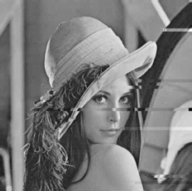
\includegraphics[width=0.42\linewidth]{images/LenaDamaged.png}
\label{fig-LenaDamaged}
}
\subfigure[Détection de la détérioration (blocs noirs)]{
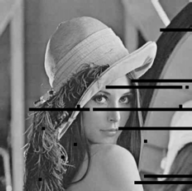
\includegraphics[width=0.42\linewidth]{images/LenaDetected.png}
\label{fig-LenaDetected}
}
\end{varwidth}}
\caption{Exemple du résultat de la détection d'erreurs avec les mesures de \citeauthor{Ye2003}
\\Tirée de \citet[p.~371]{Ye2003}}
\label{fig-LenaYe}
\end{figure}

\end{section}

\begin{section}{L'amélioration des approches d'analyse syntaxique d'encodage
vidéo}
\label{sect-SyntaxeAnalysis}
Dans le but d'améliorer l'efficacité des règles de validation de syntaxe
présentées par \citet{Talluri1998}, \citeauthor{Yan2003} proposent une nouvelle
règle de validation qui augmente considérablement l'efficacité de ce genre
d'approche. Cette règle permet de valider, entre deux marqueurs de
synchronisation, que le nombre de COD
\DIFaddbegin 

 \DIFaddend soit égal au nombre de blocs
\citep{Yan2003}. Expliquons le raisonnement derrière cette approche. Tout
d'abord, les marqueurs de synchronisation sont des séquences binaires uniques
qui servent de point de repère pour le décodeur. Le COD est un bit positionné en
début de macrobloc, qui identifie si ce dernier est encodé ou pas. Le nombre de
macroblocs contenus dans une tranche est disponible dans les paramètres
d'encodages. S'il y a eu désynchronisation, ces deux nombres risquent d'être différents\DIFaddbegin \DIFadd{,
comme illustré à la }\fig{fig-ChannelErrors}\DIFaddend .

\DIFaddbegin \begin{figure}
\DIFaddFL{\fbox{
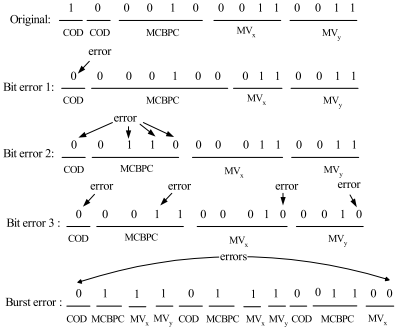
\includegraphics[width=0.65\linewidth]{images/ChannelErrors.png}
}
}\caption{\DIFaddFL{L'impact de la corruption de bits, lors du décodage.}\\\DIFaddFL{Adaptée de
}\citet[p.~1425]{Yan2003}}
\label{fig-ChannelErrors}
\end{figure}

\DIFaddend Toujours dans le même ordre d'idée, en \citeyear{Superiori2006},
\citeauthor{Superiori2006} proposent un valideur de syntaxe H.264. Ce valideur
identifie des séquences de codes binaires invalides engendrées par la
désynchronisation des codes entropiques, suite à une erreur
\citep{Superiori2006}. \DIFaddbegin \SC{Ok mais quels résultats sont obtenus par leur approche?} \DIFaddend Ce valideur est exhaustif et définit des restrictions sur
les valeurs d'un grand nombre de paramètres de la norme. \\
\\
\vbox{ \citeauthor{Superiori2006} proposent trois catégories d'erreurs de décodage selon les caractéristiques de l'erreur~\citep{Superiori2006}~:
\begin{description}
 	\item[\bul Code numérique invalide:] Il s'agit ici d'un code
 	qui n'est pas dans la table de codes numériques associés à ce paramètre.
 	\item[\bul Code hors de portée:] Lorsqu'une valeur décodée est à
 	l'extérieur de l'ensemble des valeurs valides pour le paramètre en question.
 	\item[\bul Erreur contextuelle:] Cette erreur survient si le
 	décodeur doit effectuer une opération invalide.
\end{description}
}
\end{section}

\begin{section}{La combinaison de l'analyse syntaxique et de la détection de la
détérioration visuelle dans le domaine des pixels}
\label{sect-Combined}
En \citeyear{Superiori2007}, \citeauthor{Superiori2007} combinent leur approche
de validation de syntaxe à un algorithme d'identification de la détérioration
visuelle inspiré de \citet{Ye2003}, auquel un système de vote a été ajouté, afin
\DIFdelbegin \DIFdel{d'améliorer }\DIFdelend \DIFaddbegin \DIFadd{de raffiner }\DIFaddend le résultat de la détection \citep{Superiori2007}. Dans son mémoire
\citeauthor{Ikuno2007}, explique en détail l'algorithme proposé
\citep{Ikuno2007}.

La détection de la détérioration visuelle est réalisée dans le domaine des
pixels. Pour isoler l'erreur, \citeauthor{Superiori2007} utilisent le
différentiel de la trame à évaluer par rapport à celle qui la précède (c.-à-d. la différence entre ces deux trames). La figure~\ref{fig-IkunoForeman} montre une trame endommagée ainsi que sa trame précédente. Le différentiel entre ces deux images est calculé en effectuant une différence entre les pixels correspondants (même position spatiale). Le résultat du différentiel des images de la figure~\ref{fig-IkunoForeman} est présenté à la figure~\ref{fig-Diff}.
 \DIFdelbegin \DIFdel{illustré aux figures~\ref{fig-IkunoForeman} et \ref{fig-Diff}.
}\DIFdelend \DIFaddbegin \SC{Les bonnes figures 1.4 et 1.5? Toujours présenter l'information des figures. Le lecteur ne va pas comprendre ce que tu veux qu'il comprenne. Ici 1,4 n'est pas présenté} 
\DIFaddend 

\begin{figure}
\fbox{\begin{varwidth}{\textwidth}\centering
\subfigure[Trame endommagée]{
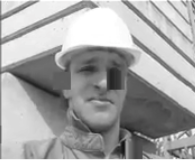
\includegraphics[width=0.42\linewidth]{images/IkunoBroken.png}
\label{fig-IkunoBroken}
}
\subfigure[Trame précédente]{
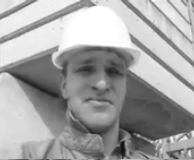
\includegraphics[width=0.42\linewidth]{images/IkunoPrev.png}
\label{fig-IkunoPrev}
}
\end{varwidth}}
\caption{Trames utilisées par \citeauthor{Ikuno2007} pour démontrer l'algorithme
de détection de la détérioration visuelle.\\Tirée de \citet[p.~25]{Ikuno2007}}
\label{fig-IkunoForeman}
\end{figure}

Par la suite, les valeurs du différentiel sont regroupées en blocs $8 \times 8$
et la moyenne est assignée comme étant représentative de l'énergie du bloc
\citep[p.~27-28]{Ikuno2007}, comme illustré à la \fig{fig-DiffAnalysis}. Les
erreurs détectées à la \fig{fig-DiffDetection} sont obtenues à l'aide d'un
seuil. Si la valeur de l'énergie d'un bloc est supérieure à ce seuil, le
bloc est considéré comme erroné.

\begin{figure}
\fbox{\begin{varwidth}{\textwidth}\centering
\subfigure[Différentiel]{
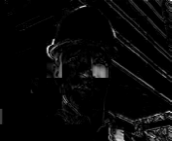
\includegraphics[width=0.30\linewidth]{images/FrameDifference.png}
\label{fig-Diff}
}
\subfigure[Analyse du différentiel]{
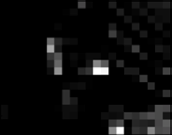
\includegraphics[width=0.30\linewidth]{images/FrameDifferenceAnalysis.png}
\label{fig-DiffAnalysis}
}
\subfigure[Erreurs détectées]{
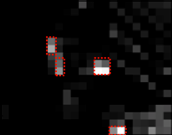
\includegraphics[width=0.30\linewidth]{images/FrameDifferenceDetection.png}
\label{fig-DiffDetection}
}
\end{varwidth}}
\caption{Exemple de l'analyse et de la detection d'erreurs.
\\Tirée de \citet[p.~25]{Ikuno2007}}
\label{fig-FrameDiff}
\end{figure}

De plus, la détection d'effets de bloc en bordure de blocs est effectuée. Pour
trouver les bordures à l'intérieur des trames, les composantes
horizontales~\ref{fig-HaarVert} et verticales~\ref{fig-HaarHori}, d'un filtre de
Haar \citep{Haar1911}, sont combinées et seulement les valeurs en bordure de
bloc sont conservées~\ref{fig-HaarCombined}. L'analyse des effets de bloc est
accomplie pour les blocs $8 \times 8$ et pour les macroblocs $16 \times 16$.
Ceux-ci sont comparés, à des seuils, afin de savoir s'il y a présence d'erreurs.

\begin{figure}
\fbox{\begin{varwidth}{\textwidth}\centering
\subfigure[Composante verticale]{
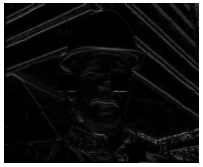
\includegraphics[width=0.42\linewidth]{images/Haar_Vert.png}
\label{fig-HaarVert}
}
\subfigure[Composante horizontale]{
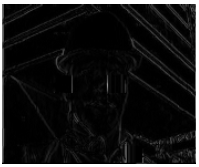
\includegraphics[width=0.42\linewidth]{images/Haar_Hori.png}
\label{fig-HaarHori}
}\\
\subfigure[Combinaison des deux composantes]{
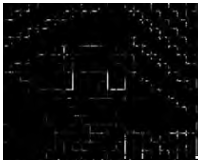
\includegraphics[width=0.42\linewidth]{images/Haar_Combined.png}
\label{fig-HaarCombined}
}
\subfigure[Analyse de bodures de blocs]{
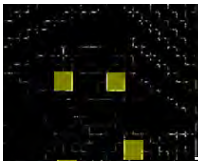
\includegraphics[width=0.42\linewidth]{images/Haar_Analysed.png}
\label{fig-HaarAnalysed}
}
\end{varwidth}}
\caption{Composantes et analyse du filtre de Haar.
\\Tirée de \citet[p.~26]{Ikuno2007}}
\label{fig-Haar}
\end{figure}

Les mesures d'énergie et d'effets de bloc sont interprétées par un système de
vote qui détermine où se trouvent les blocs erronés à l'intérieur de la trame
évaluée.

L'année suivante, \citeauthor{Farrugia2008} reprennent les travaux de
\citet{Superiori2007} et retirent les seuils et le système de vote. Ceux-ci sont 
remplacés par une machine à vecteurs de support \citep{SVM1995}. Cette dernière
est une méthode d'apprentissage supervisée qui, une fois entrainée sur un
ensemble de données, est capable de classifier d'autres données. Pour ce genre
d'algorithme, le temps d'entraînement est long, mais la classification est très
rapide, ce qui en fait un bon choix pour des considérations temps réel
\citep{Farrugia2008}.

\vbox{ Le vecteur d'entrées (\textit{feature vector}) définit par
\citeauthor{Farrugia2008} possède huit composantes: \begin{enumerate}[$\quad$1.]
\item AIDB \item La moyenne du $\text{IAIDB}_{block}$ \item L'écart type du
$\text{IAIDB}_{block}$ \item IAIDB vertical \item IAIDB horizontal \item La
moyenne du AIDSB \item L'écart type du AIDSB \item TC
\end{enumerate}
}
\begin{figure}
\fbox{\begin{varwidth}{\textwidth}\centering
\subfigure[AISDB / $\text{IAIDB}_{block}$]{
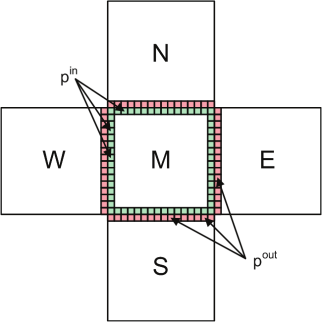
\includegraphics[width=0.30\linewidth]{images/DebonoAIDB.png}
\label{fig-DebonoAIDB}
}\hspace{0.4em}
\subfigure[IAIDB]{
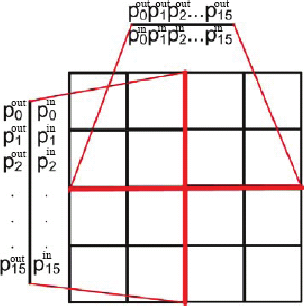
\includegraphics[width=0.30\linewidth]{images/DebonoIAIDB.png}
\label{fig-DebonoIAIDB}
}
\hspace{0.4em}
\subfigure[AIDSB]{
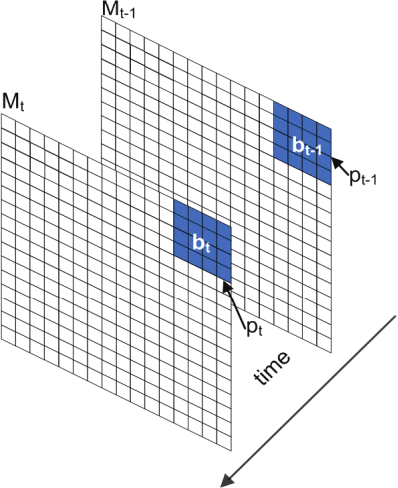
\includegraphics[width=0.30\linewidth]{images/DebonoIAIDSB.png}
\label{fig-DebonoAIDSB}
}
\end{varwidth}}
\caption{Visualisation des composantes du vecteur d'entrées.
\\Tirée de \citet[p.~79-80]{Farrugia2010}}
\DIFdelbeginFL %DIFDELCMD < \label{fig-Debono}
%DIFDELCMD < %%%
\DIFdelendFL %DIF >  \label{fig-IkunoForeman}
\end{figure}
\DIFaddbegin 

\SC{Expliciter tous les acronymes. Aussi la figure montre AISDB et tu parles de AIDB partout, c'est quoi la relation?}

\DIFaddend Ce vecteur représente un macrobloc contenu à l'intérieur d'une trame d'une
séquence vidéo. Le AIDB est la différence moyenne des pixels en bordure de
macroblocs (M, à la \fig{fig-DebonoAIDB}). Le $\text{IAIDB}_{block}$ est la même
mesure que le AIDB, mais appliquée aux blocs $4 \times 4$ à l'intérieur d'un
macrobloc. Le IAIDB est la moyenne de la différence des pixels pour les bordures
internes (verticales et horizontales) d'un macrobloc (lignes rouges
\fig{fig-DebonoIAIDB}). Le AIDSB est l'énergie d'un macrobloc $16 \times 16$,
tel que défini par \citet{Ikuno2007}, soit la moyenne du différentiel par
rapport à la trame précédente (voir la \fig{fig-DebonoAIDSB}). La consistance de
la texture (TC) est basée sur une approche d'analyse de texture présentée par
\citet{Wang1990} connue sous le nom de patron binaire local \ang{Local Binary
Pattern (LBP)}.
\end{section}
\DIFaddbegin \SC{Résultats de cette aproche? performace?}

\SC{IMPORTANT: Dans un chapitre sur l'état de l'art, on s'attend à avoir une analyse critique des méthodes existantes avec leurs performances, leurs points forts et leurs points faibles. Cela sert à justifier pourquoi on choisit une approche différente.}

\SC{Revoir les références, il manque des accents à décembre. Revoir Ikunu 2007 car accent mal placé et 'master thesis' à franciser. REvoir avec la tite dame les question de référence et traduction de 'in proceeding' , 'in', ...}
\DIFaddend 

En somme, ce chapitre offre un bref survol des travaux de recherche en lien
avec~: le \textit{Joint Source Channel Decoding}, la résilience aux erreurs lors
du transport de vidéo, la validation de syntaxe pour les normes d'encodage vidéo
et la détection de la détérioration visuelle dans le domaine des pixels. Ces
concepts sont présentés dans un ordre quasi chronologique, où la cohésion
conceptuelle a raison de la chronologie. Conséquemment, ils servent
de notions fondatrices aux approches proposées dans cet ouvrage, et présentées
dans le prochain chapitre.


\end{chapter}

\bibliographystyle{bibETS}
\bibliography{revuelit}
\end{document}
